\documentclass[12pt]{beamer}
\usetheme{Malmoe}
\usepackage{siunitx}
\usepackage{hyperref}
\usepackage{cancel}
\sisetup{
  per-mode = fraction,
  fraction-function = \frac
}

\begin{document}


\title{Paper Presentation: Depth Anything}
\subtitle{\begin{itemize}
        \item Depth Anything: Unleashing the Power of Large-Scale Unlabeled Data
        \item Depth Anything V2
    \end{itemize}}
\author{Benjamin Stadler}
\institute{Tsinghua University \\
    Machine Vision (Fall 2024) \\
Contact: \texttt{\href{mailto:bestadle@ethz.ch}{bestadle@ethz.ch}}}
\date{October 2024}


\begin{frame}
\titlepage
\end{frame}


\begin{frame}
    \frametitle{At a Glace}

    \begin{itemize}
        \item[What] Molecular Depth Estimation (MDE)
        \item[Who] HKU, TikTok
        \item[When] April 2024 (V1), June 2024 (V2)
        \item[How] train with \underline{unlabeled data} $\implies$ improve state-of-the-art
    \end{itemize}
    
    \begin{figure}
        \centering
        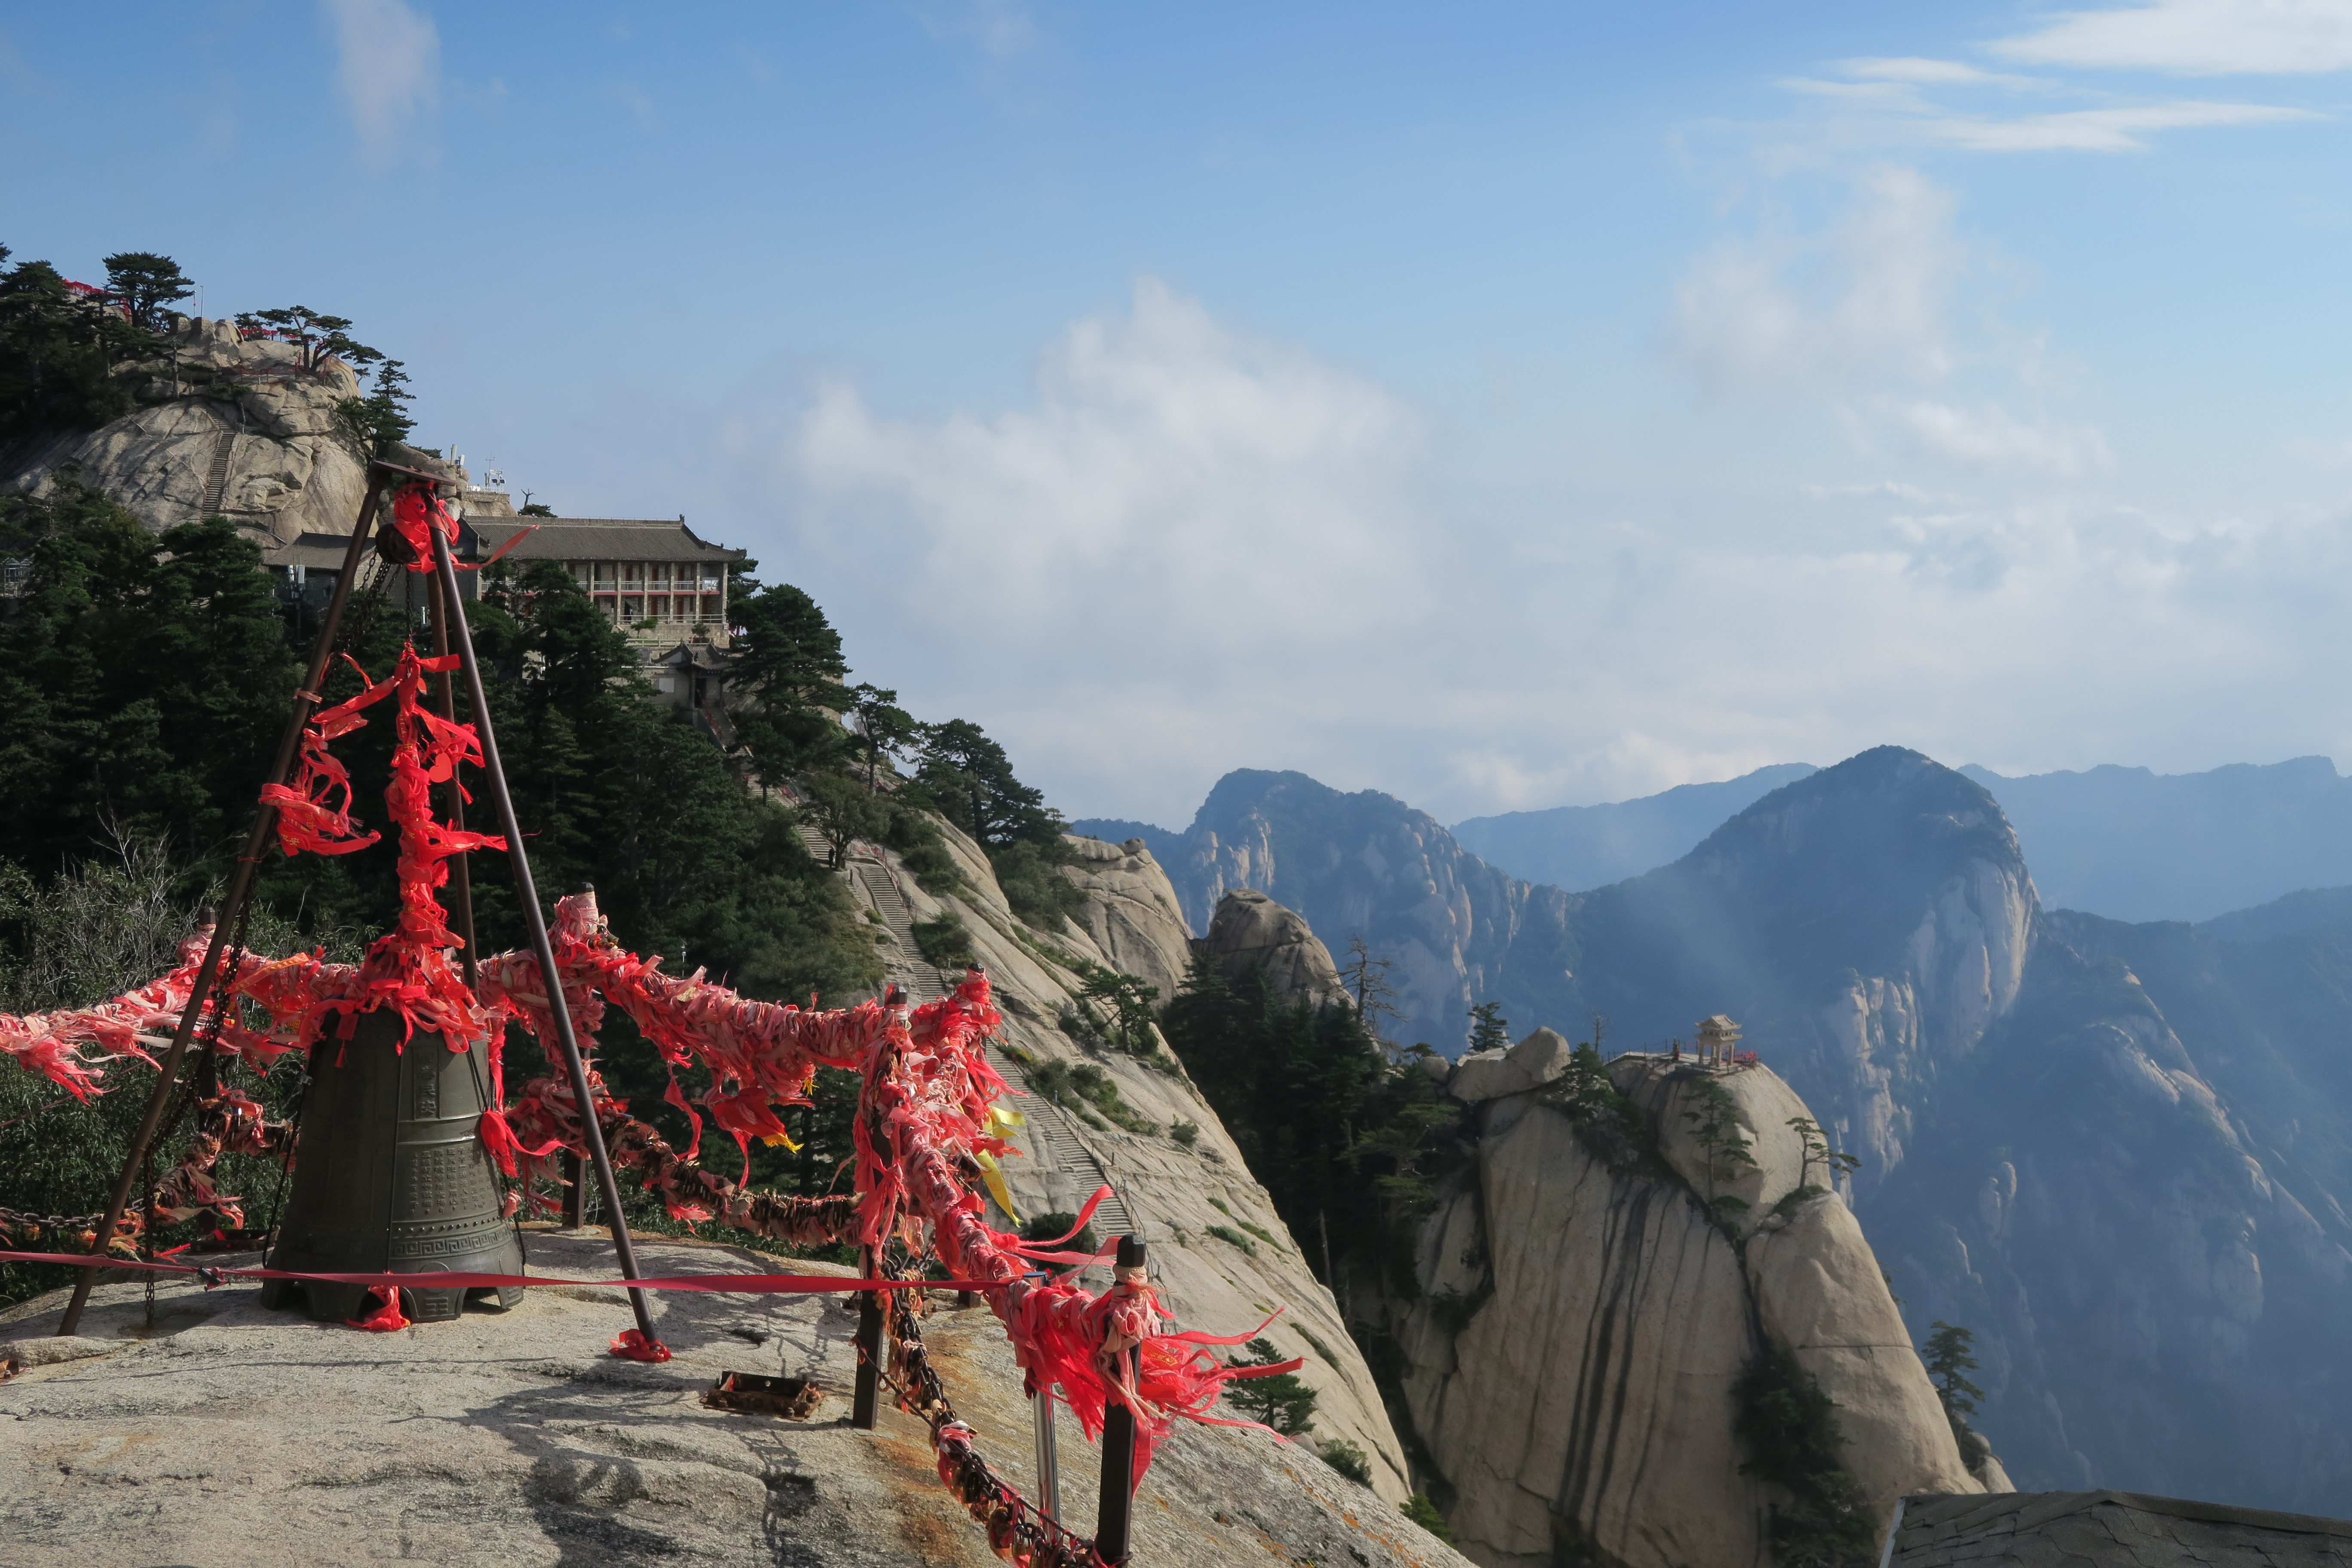
\includegraphics[width=0.45\textwidth]{./figures/huashan_orig.jpg}
        \includegraphics[width=0.45\textwidth]{./figures/huashan_depthmap.png}
        \caption{Sample Input $\to$ Output (V2, large model)}
        \label{fig:intro}
    \end{figure}

\end{frame}


\begin{frame}
    \frametitle{Sources}
    \tiny
    
    \textbf{Presentation \& Code} \href{https://github.com/birawaich/thu_mavi_paperpresentation}{Github}
    
    \textbf{Papers}
    \begin{itemize}
        \item \href{https://arxiv.org/abs/2401.10891}{Depth Anything: Unleashing the Power of Large-Scale Unlabeled Data}
        \item \href{https://arxiv.org/abs/2406.09414}{Depth Anything V2}
    \end{itemize}
    
    \textbf{Pictures}
    if not noted differently, own captions.
    
    
\end{frame}

\end{document}
